\section{Tiền xử lý số liệu}
    Trong phần Tiền xử lý dữ liệu, nhóm sử dụng môi trường lập trình \textbf{R} và giao diện \textbf{RStudio} làm công cụ xử lý dữ liệu gốc. Để chuẩn bị dữ liệu đầu vào chuẩn xác và có độ tin cậy cao cho các phân tích thống kê mô tả cũng như hồi quy tuyến tính ở các phần sau, nhóm tiến hành quy trình tiền xử lý dữ liệu qua 4 giai đoạn cụ thể dưới đây.

    \subsection{Trích lọc tập biến quan tâm}
        Bộ dữ liệu ban đầu \texttt{All\_GPUs.csv} gồm 3,406 mẫu quan sát và 34 biến thông số kỹ thuật. Nhóm lọc ra 9 thông số kỹ thuật phần cứng cốt lõi nhất đại diện cho năng lực xử lý nhân và hệ thống bộ nhớ GPU, đồng thời giữ lại biến định danh tên sản phẩm (\texttt{Name}) để phục vụ bước lọc trùng lặp:

        \begin{itemize}
            \item \textbf{Biến định danh}: \texttt{Name} (Tên mẫu card đồ họa).
            \item \textbf{Biến nhân xử lý}: \texttt{Core\_Speed} (MHz), \texttt{Max\_Power} (Watts), \texttt{Process} (nm), \texttt{ROPs}, \texttt{TMUs}.
            \item \textbf{Biến hệ thống bộ nhớ}: \texttt{Memory} (MB), \texttt{Memory\_Bandwidth} (GB/s), \texttt{Memory\_Bus} (Bit), \texttt{Memory\_Speed} (MHz).
        \end{itemize}

        Đọc dữ liệu bằng hàm \texttt{read.csv()} của R, chuẩn hóa các chuỗi đại diện cho dữ liệu khuyết như \texttt{"\textbackslash n-"}, \texttt{"-"}, \texttt{"None"}, \texttt{""} thành \texttt{NA}.

        \begin{figure}[H]
            \centering
            \begin{subfigure}[b]{0.92\textwidth}
                \centering
                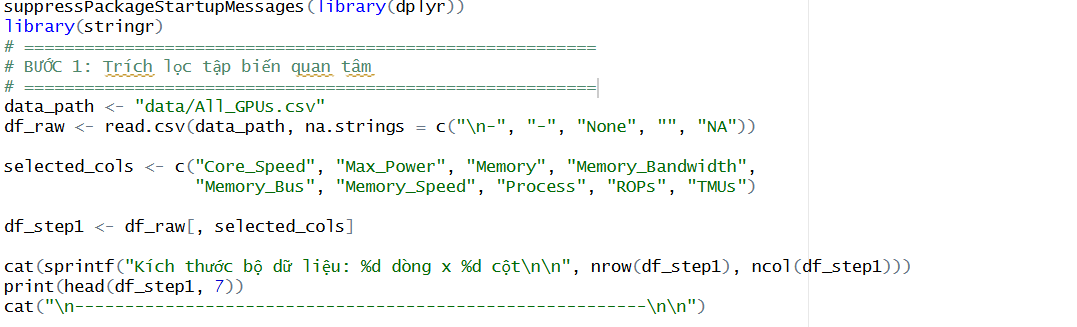
\includegraphics[width=\textwidth]{dataPrep/m1a.png}
            \end{subfigure}
            \vspace{0.4cm}
            \begin{subfigure}[b]{0.92\textwidth}
                \centering
                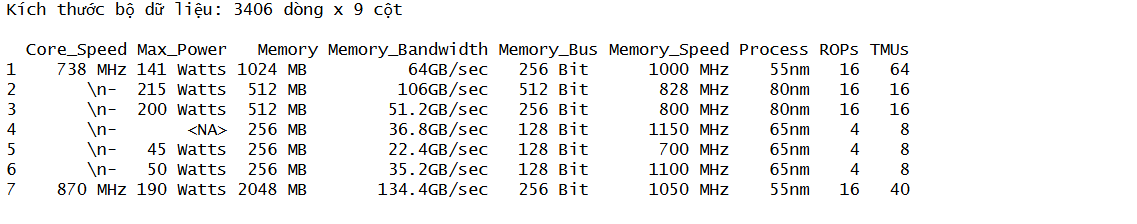
\includegraphics[width=\textwidth]{dataPrep/m1b.png}
            \end{subfigure}
            \caption{Kết quả trích lọc tập biến quan tâm}
            \label{fig:Trích lọc tập biến quan tâm}
        \end{figure}

    \subsection{Tách bỏ đơn vị, quy đổi hệ số và chuyển đổi kiểu dữ liệu}
        Dữ liệu gốc chứa các ký tự đơn vị và hậu tố đi kèm. Nhóm sử dụng thư viện \texttt{stringr} để trích xuất giá trị số thực và chuẩn hóa đồng nhất đơn vị cho toàn bộ 9 cột về kiểu dữ liệu số (\texttt{numeric}):
        \begin{itemize}
            \item \textbf{Chuẩn hóa băng thông (\texttt{Memory\_Bandwidth}):} Một số dòng GPU đời cũ sử dụng đơn vị \texttt{MB/sec} thay vì \texttt{GB/sec}. Nhóm thực hiện nhận diện chuỗi \texttt{"MB"} và chia cho $1024$ để quy đổi toàn bộ cột về chung đơn vị chuẩn \texttt{GB/sec}.
            \item \textbf{Xử lý hậu tố nhân đơn vị (\texttt{ROPs}, \texttt{TMUs}):} Các cấu hình GPU nhân đôi (Dual-GPU) có giá trị dạng \texttt{16 (x2)}. Hệ thống tự động tách phần số gốc và nhân với hệ số trong ngoặc (ví dụ: $16 \times 2 = 32$) để phản ánh đúng tổng năng lực phần cứng thực tế.
            \item \textbf{Các biến còn lại:} Loại bỏ các hậu tố \texttt{MHz}, \texttt{Watts}, \texttt{MB}, \texttt{Bit}, \texttt{nm} và ép kiểu sang \texttt{numeric}.
        \end{itemize}

        \begin{figure}[H]
            \centering
            \begin{subfigure}[b]{0.92\textwidth}
                \centering
                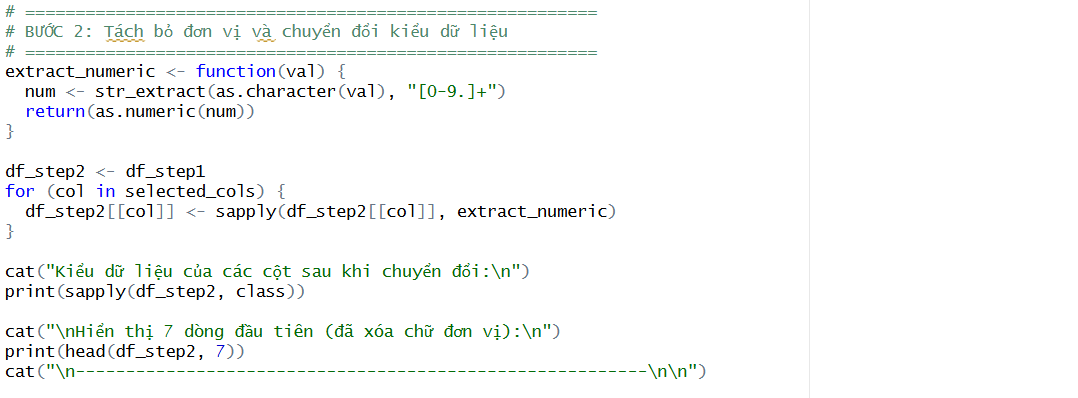
\includegraphics[width=\textwidth]{dataPrep/m2a.png}
            \end{subfigure}
            \vspace{0.4cm}
            \begin{subfigure}[b]{0.92\textwidth}
                \centering
                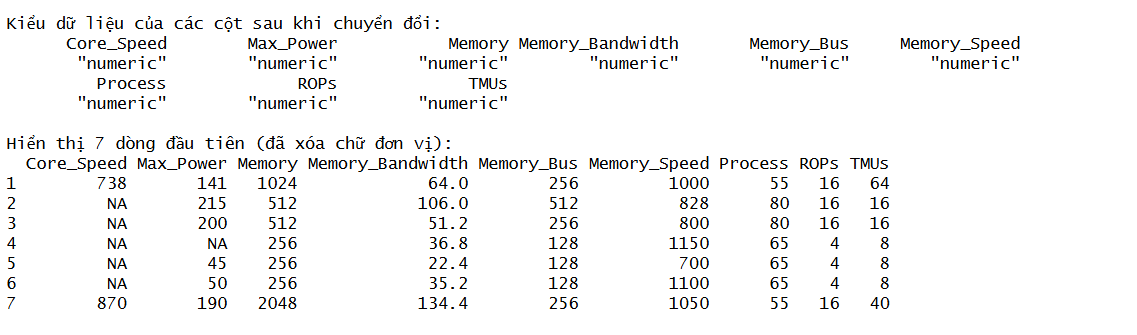
\includegraphics[width=\textwidth]{dataPrep/m2b.png}
            \end{subfigure}
            \caption{Kết quả tách bỏ đơn vị và chuyển đổi kiểu dữ liệu}
            \label{fig:Tách bỏ đơn vị và chuyển đổi kiểu dữ liệu}
        \end{figure}

    \subsection{Chuẩn hóa ô trống và xử lý dữ liệu khuyết}
        Dữ liệu khuyết trong tập dữ liệu mang đặc tính không hoàn toàn ngẫu nhiên (MAR/MNAR) do các dòng GPU đời cũ hoặc chip tích hợp thường không công bố đầy đủ thông số. Do các thông số phần cứng mang tính kiến trúc cố định, việc thay thế dữ liệu (Imputation) bằng giá trị trung bình/trung vị có thể làm bóp méo bản chất kỹ thuật. Nhóm áp dụng phương pháp \textbf{Loại bỏ theo dòng (Listwise Deletion)} bằng hàm \texttt{na.omit()}.

        \begin{figure}[H]
            \centering
            \begin{subfigure}[b]{0.92\textwidth}
                \centering
                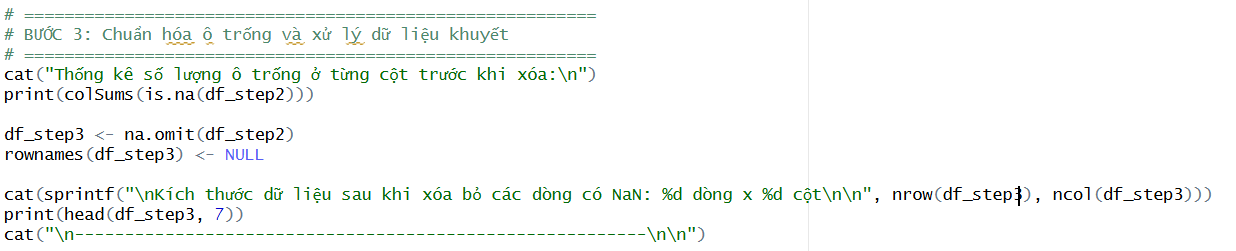
\includegraphics[width=\textwidth]{dataPrep/m3a.png}
            \end{subfigure}
            \vspace{0.4cm}
            \begin{subfigure}[b]{0.92\textwidth}
                \centering
                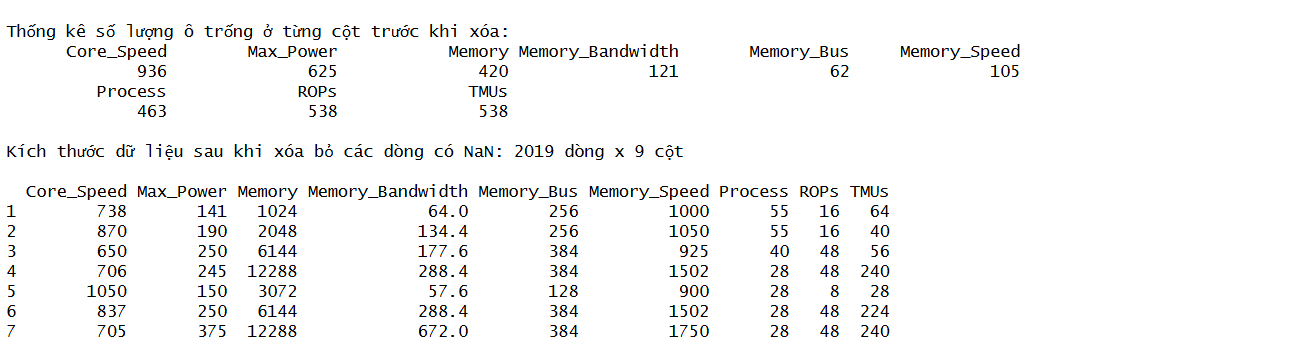
\includegraphics[width=\textwidth]{dataPrep/m3b.png}
            \end{subfigure}
            \caption{Kết quả thống kê ô trống và loại bỏ dữ liệu khuyết}
            \label{fig: Chuẩn hóa ô trống và xử lý dữ liệu khuyết}
        \end{figure}

    \subsection{Loại bỏ quan sát trùng lặp theo từng mẫu GPU}
        Trong thực tế phần cứng, hai mẫu card đồ họa khác tên (ví dụ các phiên bản thương mại khác nhau hoặc khác dòng sản phẩm) vẫn có thể sở hữu bộ 9 thông số kỹ thuật giống nhau. Nếu lọc trùng dựa trên 9 thông số sẽ vô tình làm mất đi các quan sát hợp lệ. Do đó, nhóm thực hiện lọc trùng dựa trên biến định danh tên sản phẩm (\texttt{Name}) bằng hàm \texttt{distinct(Name, .keep\_all = TRUE)} thuộc gói \texttt{dplyr} để đảm bảo mỗi dòng đại diện cho một mẫu GPU duy nhất, sau đó mới loại bỏ cột \texttt{Name} để thu được bảng dữ liệu định lượng sạch hoàn chỉnh.

        \begin{figure}[H]
            \centering
            \begin{subfigure}[b]{0.92\textwidth}
                \centering
                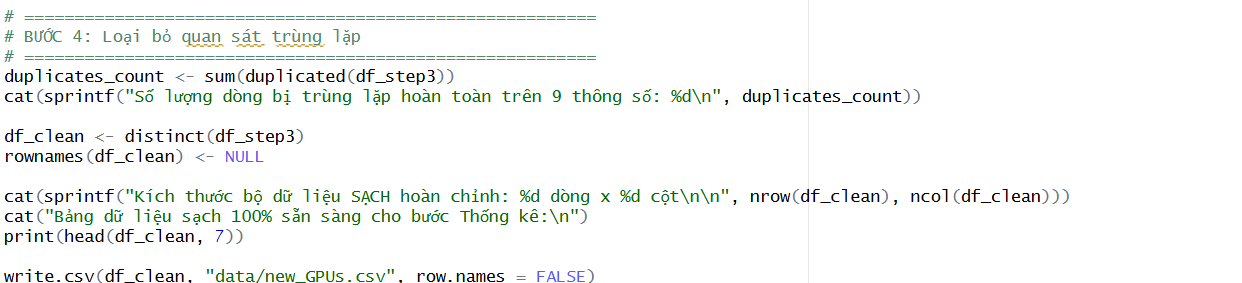
\includegraphics[width=\textwidth]{dataPrep/m4a.png}
            \end{subfigure}
            \vspace{0.4cm}
            \begin{subfigure}[b]{0.92\textwidth}
                \centering
                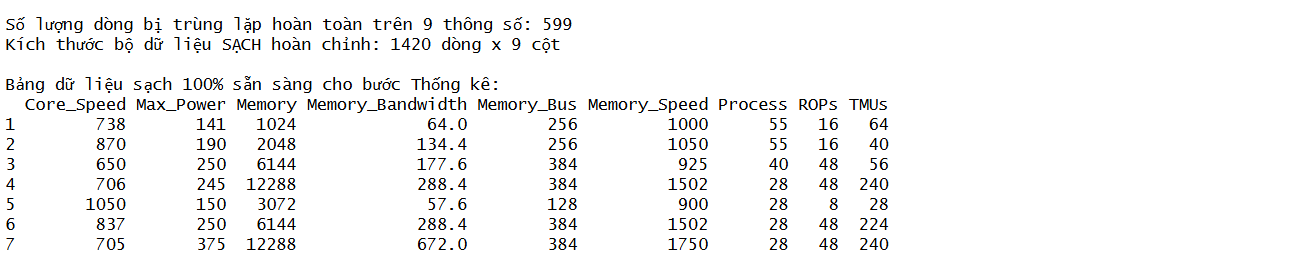
\includegraphics[width=\textwidth]{dataPrep/m4b.png}
            \end{subfigure}
            \caption{Kết quả loại bỏ quan sát trùng lặp theo tên GPU}
            \label{fig:Loại bỏ quan sát trùng lặp}
        \end{figure}

    \subsection{Mã nguồn xử lý bằng R}
        Đoạn mã R thực hiện trọn vẹn 4 giai đoạn tiền xử lý:

\begin{pythoncode}
suppressPackageStartupMessages(library(dplyr))
library(stringr)

# BUOC 1: Trich loc 9 bien quan tam kem bien dinh danh Name
df_raw <- read.csv('data/All_GPUs.csv', na.strings = c('\n-', '-', 'None', '', 'NA'))
selected_cols <- c('Core_Speed', 'Max_Power', 'Memory', 'Memory_Bandwidth', 
                   'Memory_Bus', 'Memory_Speed', 'Process', 'ROPs', 'TMUs')
df_step1 <- df_raw[, c('Name', selected_cols)]

# BUOC 2: Tach don vi, quy doi MB/s -> GB/s va nhan he so (x2)
extract_numeric <- function(val) as.numeric(str_extract(as.character(val), '[0-9.]+'))

parse_bandwidth <- function(val) {
  str_val <- as.character(val)
  num <- as.numeric(str_extract(str_val, '[0-9.]+'))
  is_mb <- str_detect(str_val, regex('MB', ignore_case = TRUE))
  ifelse(!is.na(num) & !is.na(is_mb) & is_mb, num / 1024, num)
}

parse_units_multiplier <- function(val) {
  str_val <- as.character(val)
  base_num <- as.numeric(str_extract(str_val, '^[0-9.]+'))
  mult_str <- str_extract(str_val, '(?<=\\(x)[0-9.]+(?=\\))')
  mult <- ifelse(is.na(mult_str), 1, as.numeric(mult_str))
  return(base_num * mult)
}

df_step2 <- df_step1
for (col in selected_cols) {
  if (col == 'Memory_Bandwidth') {
    df_step2[[col]] <- parse_bandwidth(df_step2[[col]])
  } else if (col %in% c('ROPs', 'TMUs')) {
    df_step2[[col]] <- parse_units_multiplier(df_step2[[col]])
  } else {
    df_step2[[col]] <- sapply(df_step2[[col]], extract_numeric)
  }
}

# BUOC 3: Xu ly du lieu khuyet (Listwise Deletion)
df_step3 <- na.omit(df_step2)

# BUOC 4: Loai bo trung lap theo ten mau GPU (Name)
df_step3$Name <- str_trim(as.character(df_step3$Name))
df_clean <- df_step3 %>%
  distinct(Name, .keep_all = TRUE) %>%
  select(all_of(selected_cols))

write.csv(df_clean, 'data/new_GPUs.csv', row.names = FALSE)
\end{pythoncode}